\documentclass[11pt]{article}
\usepackage{acl}
\usepackage{times}
\usepackage{latexsym}
\usepackage[T1]{fontenc}
\usepackage[utf8]{inputenc}
\usepackage{microtype}
\usepackage{inconsolata}
\usepackage{amsmath,amssymb,mathtools}
\usepackage{graphicx}
\usepackage{booktabs}
\usepackage{xcolor}
\usepackage{subcaption}
\usepackage{xspace}
\usepackage{multirow}
\usepackage{array}
\usepackage{placeins}

% Math commands
\newcommand{\method}{\textsc{RWS}\xspace}
\newcommand{\longmethod}{Route-Weighted Sensitivity\xspace}
\newcommand{\rhi}{\mathrm{RHI}}
\newcommand{\piprob}{\pi}
\newcommand{\Loss}{\mathcal{L}}
\DeclareMathOperator*{\argmin}{arg\,min}
\newcommand{\abs}[1]{\lvert #1 \rvert}

\title{Route-Weighted Sensitivity for Mixed-Precision \\ MoE Quantization}

\author{Anonymous}
\date{}

\begin{document}
\maketitle

\begin{abstract}
Mixed-precision post-training quantization of Mixture-of-Experts (MoE) language models allocates different bit-widths to different expert weight blocks by solving a constrained optimization over per-block sensitivity scores. We identify a structural mismatch in how this problem is \emph{scored}: existing allocators weight every expert's reconstruction loss equally, yet MoE routing is inherently sparse and skewed---a few experts process most tokens. We propose \longmethod (\method), which scales each expert's sensitivity by a routing-aware weight before feeding it to the allocator. The method requires no tuning or additional compute beyond the standard calibration pass, and drops into any sensitivity-based allocation pipeline. We also introduce the Route Heterogeneity Index ($\rhi$), a preliminary diagnostic scalar that quantifies routing skew. Experiments on three MoE architectures (Qwen1.5-MoE, Mixtral-8x7B, DeepSeek-MoE) show that \method\ reduces WikiText-2 perplexity by up to 2.8\% at 2.5 bits/parameter and improves downstream accuracy by up to +0.7 percentage points, with consistent gains across all three models. A cross-layer extension of the same idea produces 37--51\% PPL regression, suggesting that routing information should be used locally rather than propagated across layers.
\end{abstract}

\section{Introduction}
\label{sec:intro}

Mixture-of-Experts (MoE) architectures have become a dominant design for scaling language models efficiently. Models such as Mixtral-8x7B \citep{jiang2024mixtral}, Qwen1.5-MoE \citep{bai2023qwen}, DeepSeek-V3 \citep{deepseekai2024deepseekv3}, and Switch Transformers \citep{fedus2022switch} place 80--95\% of their parameters in expert feed-forward blocks, while activating only a sparse subset per token through a learned router \citep{shazeer2017outrageously,lepikhin2021gshard}. This sparsity creates an opportunity for efficient serving, but also poses a challenge for post-training quantization: the bit-allocation problem---\emph{how many bits to assign each expert}---must respect a global budget while minimizing output quality degradation \citep{duanmu2025mxmoe,li2024quantmoebench,frantar2023qmoe}.

Sensitivity-based allocators solve this by measuring per-block reconstruction loss under each candidate quantization strategy and selecting the assignment that minimizes total loss subject to a bit budget \citep{yao2021hawqv3,duanmu2025mxmoe}. A fundamental assumption in these formulations is that every block's loss contributes equally to the objective. For dense transformers this is reasonable; for MoE models it is not. Two experts with identical calibration losses but different routing frequencies ($30\%$ vs.\ $0.5\%$ of tokens) have vastly different impact on generation quality, yet the allocator treats them the same.

We propose \longmethod (\method), a modification to the allocation objective that combines two orthogonal information sources: per-block quantization sensitivity (which blocks suffer from low-bit quantization) and empirical routing frequency (which blocks matter most at inference). Before the solver runs, we scale each expert's sensitivity by a routing-aware weight. The modification requires no tuning of weighting strength or additional calibration data, and uses only routing statistics already collected during calibration.

We additionally introduce the \emph{Route Heterogeneity Index} ($\rhi$), a scalar derived from the routing trace that quantifies how skewed the expert access distribution is:
\begin{equation}
\label{eq:rhi_intro}
  \rhi \;=\; \frac{1}{L}\sum_{l=1}^{L}
    \bigl[\log N - H\!\bigl(\piprob_l\bigr) + 1\bigr],
\end{equation}
where $H$ is Shannon entropy, $N$ is the number of routed experts, and $\piprob_l$ is the normalized access-frequency vector at layer~$l$. A model with uniform routing has $\rhi\!=\!1$; higher values indicate greater skew and, we hypothesize, greater leverage for \method.

Our contributions are:
\begin{enumerate}
\item \textbf{\method} (\S\ref{sec:method}): route-weighted sensitivity for ILP-based mixed-precision allocation. Zero hyperparameters, zero extra compute, drop-in compatible.
\item \textbf{Route Heterogeneity Index} (\S\ref{sec:rhi}): a preliminary diagnostic scalar that quantifies routing skew and is consistent with the direction of \method\ gains in our experiments.
\item \textbf{Empirical validation} (\S\ref{sec:results}): on three MoE architectures---Qwen1.5-MoE-A2.7B ($\rhi\!=\!1.84$), Mixtral-8x7B ($\rhi\!=\!1.84$), and DeepSeek-MoE-16B ($\rhi\!=\!1.56$)---\method\ reduces WikiText-2 PPL by $2.8\%$, $1.0\%$, and $1.3\%$ respectively at 2.5\,bits/param, with consistent downstream accuracy improvements.
\item \textbf{Negative result} (\S\ref{sec:results}): a cross-layer propagation extension regresses PPL by 37--51\%, suggesting that routing information should be used locally.
\end{enumerate}

\section{Background}
\label{sec:background}

\subsection{Mixture-of-Experts}

An MoE layer consists of $N$ expert sub-networks $\{E_e\}_{e=1}^{N}$ and a learnable router $R$ \citep{shazeer2017outrageously}. For an input token $x$, the router produces logits $\ell = R(x) \in \mathbb{R}^N$; a top-$k$ mechanism selects indices $\mathcal{T}(x) \subset [N]$ and assigns normalized weights $w_e(x) = \mathrm{softmax}(\ell)_e$ for $e \in \mathcal{T}(x)$. The layer output is a weighted combination:
\begin{equation}
\label{eq:moe}
  y \;=\; \sum_{e \in \mathcal{T}(x)} w_e(x)\, E_e(x).
\end{equation}
The routing distribution $\piprob_l \in \Delta^{N-1}$ at layer $l$ is defined as the normalized frequency with which each expert appears in the top-$k$ set over a calibration corpus. In practice, $\piprob_l$ is highly non-uniform: a small subset of experts receives the majority of routing mass \citep{fedus2022switch,zoph2022stmoe}.

\subsection{Mixed-Precision Quantization for MoE}

Post-training quantization (PTQ) reduces a model's memory footprint by replacing full-precision weights with low-bit representations \citep{frantar2023gptq,lin2024awq,xiao2023smoothquant,dettmers2022llmint8}. For MoE models, the key question is \emph{mixed-precision allocation}: assigning different bit-widths to different expert blocks to minimize output degradation under a global bit budget.

A standard pipeline proceeds in three stages:
\begin{enumerate}
\item \textbf{Calibration.} A small dataset $\mathcal{D}_{\mathrm{cal}}$ (e.g., 128 samples from WikiText-2) is used to measure per-block reconstruction loss $\Loss_{b,s}$ for each candidate strategy $s \in \mathcal{S}$ and each linear block $b$.
\item \textbf{Allocation.} An optimizer (typically ILP \citep{yao2021hawqv3} or greedy search) solves:
\begin{align}
\label{eq:ilp}
  \min_{x_{b,s} \in \{0,1\}} \;&\sum_{b,\,s} \Loss_{b,s}\, x_{b,s} \\
  \text{s.t.}\quad
  &\sum_{s} x_{b,s} = 1 \;\;\forall\, b, \nonumber\\
  &\sum_{b,\,s} \mathrm{bits}_s \cdot \abs{b} \cdot x_{b,s} \le B, \nonumber
\end{align}
where $B$ is the total bit budget and $\abs{b}$ is the parameter count of block $b$.
\item \textbf{Quantization.} The chosen per-block strategies are applied using RTN, GPTQ \citep{frantar2023gptq}, or similar methods.
\end{enumerate}

Recent work extends this framework to MoE with hardware-aware ILP formulations \citep{duanmu2025mxmoe,li2024quantmoebench}. MxMoE \citep{duanmu2025mxmoe} adds a latency penalty and expert-aware GroupGEMM kernels. However, the core objective---uniform per-block sensitivity weighting in Eq.~\ref{eq:ilp}---remains unchanged.

\subsection{The Routing--Sensitivity Gap}

Equation~\ref{eq:ilp} treats every block identically: a rarely-activated expert with loss $\Loss$ contributes the same amount to the objective as a frequently-activated expert with the same $\Loss$. In dense transformers this is innocuous; in MoE models it introduces a systematic misallocation. Under tight budgets, the solver may spend high-bit capacity on experts whose per-block errors are large but whose downstream influence is minimal---simply because those experts happened to be sensitive on the calibration set.
\section{Method}
\label{sec:method}

\begin{figure*}[t]
\centering
% Placeholder for user's hand-drawn framework figure
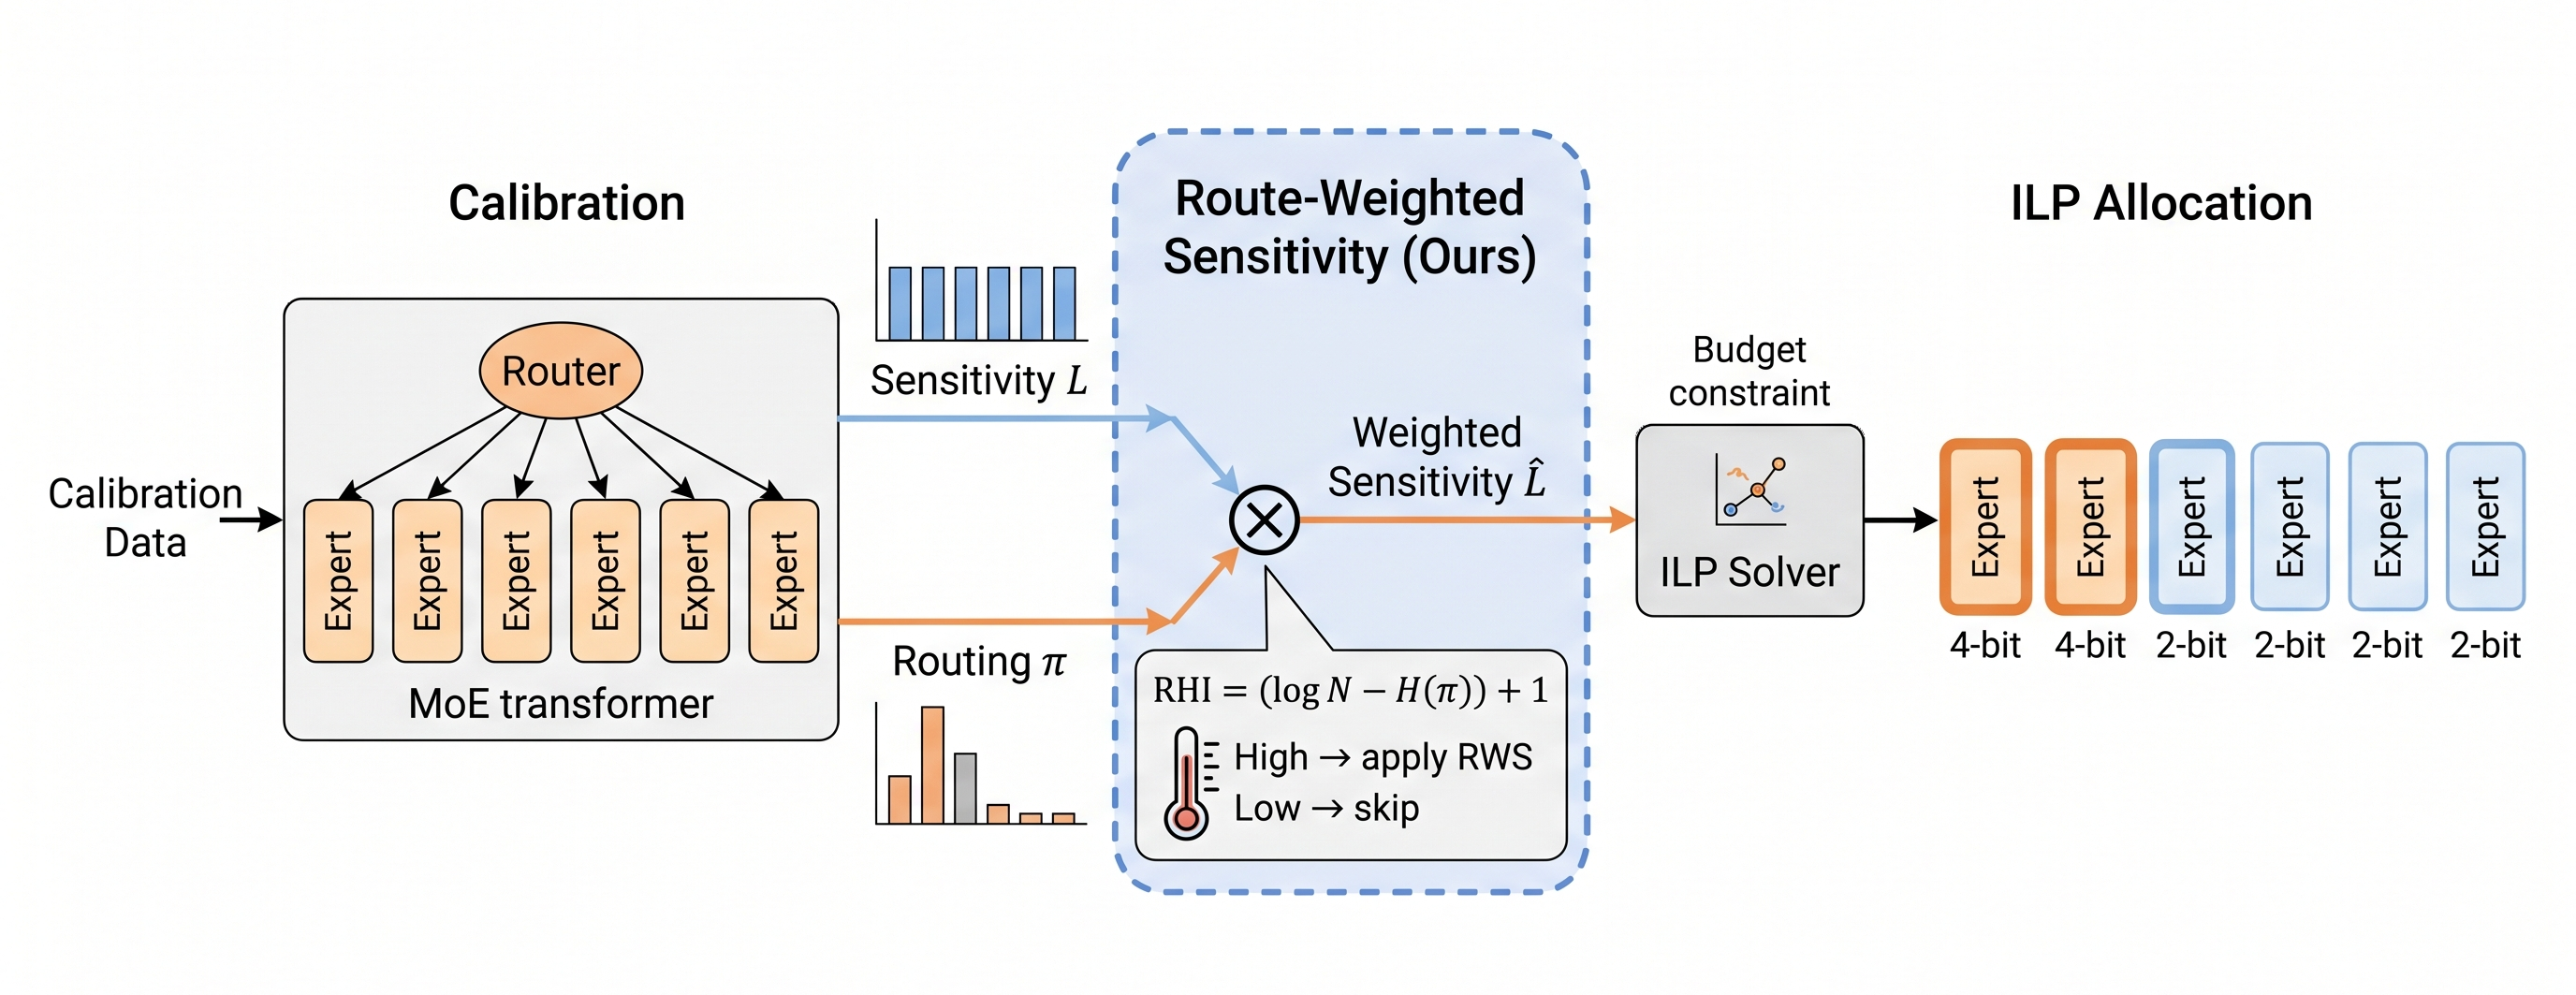
\includegraphics[width=0.95\textwidth]{figures/fig_framework.png}
\caption{Overview of \method. During the calibration forward pass, we collect both per-expert sensitivity scores $\Loss_{b,s}$ and routing probabilities $\piprob_{l,e}$. \method\ weights each expert's sensitivity by $\piprob_{l,e}$ before feeding it to the ILP allocator.}
\label{fig:framework}
\end{figure*}

\subsection{Route-Weighted Sensitivity}

Let $\piprob_{l,e} \in [0,1]$ denote the empirical routing probability of expert $e$ in layer $l$---the fraction of calibration tokens for which $e \in \mathcal{T}(x)$. Define the per-layer normalized routing weight:
\begin{equation}
\label{eq:weight}
  w_{l,e} \;=\; \frac{\piprob_{l,e}}{\max_{e'}\, \piprob_{l,e'}} \;\in\; [0,\, 1].
\end{equation}
We modify each block's sensitivity before the ILP by applying:
\begin{equation}
\label{eq:rws}
  \hat{\Loss}_{b,s} \;=\; \Loss_{b,s} \cdot \bigl(1 + w_{l(b),\,e(b)}\bigr).
\end{equation}
The $(1 + w)$ form ensures that high-frequency experts (with $w \approx 1$) receive approximately doubled sensitivity, while the lowest-frequency experts retain their original loss unchanged. The ILP then minimizes $\sum_{b,s} \hat{\Loss}_{b,s}\, x_{b,s}$ subject to the same constraints as Eq.~\ref{eq:ilp}. The substitution changes \emph{only} the objective; the constraints, strategy pool, solver, and calibration data are identical.

\paragraph{Loss computation.}
The calibration loss $\Loss_{b,s}$ is computed as follows. During the calibration forward pass, every expert processes \emph{all} calibration inputs regardless of routing. For each expert's linear block (gate, up, or down projection), we quantize the block weights to strategy $s$ and compute the $\ell_2$ reconstruction error $\|\hat{y} - y\|_2$ between the quantized and full-precision block outputs, averaged over the calibration sequence. This is an \emph{unconditional} per-block loss: it does not distinguish between tokens that are and are not routed to the expert. This distinction matters because the unconditional loss treats all blocks equally, while the expected inference loss weights each block by the probability that it is actually used. \method\ bridges this gap by scaling the unconditional loss by routing frequency.

\paragraph{Why $(1 + w)$ rather than raw $\piprob$.}
A theoretically cleaner objective would multiply by raw $\piprob_{l,e}$ to approximate the expected routed-token loss. We use the $(1 + w)$ form because it is conservative: it boosts high-frequency experts by at most $2\times$ and never reduces any expert's loss below its baseline. The $(1 + w)$ form recovers the baseline when routing is uniform ($w\!=\!1$ for all experts). While $(1 + w)$ and raw $\piprob$-weighting are both monotone in $\piprob$, they do not necessarily produce the \emph{same} ILP allocation in general, because the ILP's budget constraint creates tradeoffs across layers and blocks where the magnitude of the scaling---not just the ranking---affects which marginal block is promoted or demoted. In practice, we observe nearly identical allocations: on Qwen at 2.5\,bits, the two formulations differ in only 3 of 1,464 blocks.

\paragraph{Approximation caveat.}
The true conditional loss for expert $e$ is $\mathbb{E}_{x:\, e \in \mathcal{T}(x)}[\Loss_{e,s}(x)]$, which decomposes as $\Pr(e \in \mathcal{T}) \cdot \mathbb{E}_x[\Loss_{e,s}(x)]$ only when the quantization error is independent of whether $e$ is selected. When experts specialize \citep{zhou2022expertchoice}, this independence is imperfect. RWS is therefore a \emph{first-order approximation}. Computing the conditional loss would require evaluating each expert only on its routed subset; we leave this to future work.

\paragraph{Selection frequency vs.\ gate weight.}
We use $\piprob_{l,e} = \Pr(e \in \mathcal{T}(x))$ (top-$k$ selection frequency) rather than the expected gate weight $\alpha_{l,e} = \mathbb{E}_x[\mathbf{1}(e \in \mathcal{T}(x)) \cdot w_e(x)]$. The two are correlated but not identical; we choose $\piprob$ because it is simpler and produces nearly identical results (PPL 9.35 vs.\ 9.34 at 2.5\,b on Qwen). This ablation on Qwen shows that the specific choice of routing statistic matters less than the presence of routing information in the objective.

\paragraph{Shared experts.}
Models with shared experts (Qwen: 1 shared + 60 routed; DeepSeek: 2 shared + 64 routed) always activate their shared experts. Since shared experts have no routing decision, $\piprob$ is undefined for them. We apply route weighting \emph{only} to routed expert blocks, leaving shared expert sensitivities at their original values ($\hat{\Loss}_{b,s} = \Loss_{b,s}$). Mixtral has no shared experts, so all blocks are route-weighted.

\subsection{Route Heterogeneity Index}
\label{sec:rhi}

\method\ has leverage only when $\piprob$ is non-uniform. We quantify routing skew with the \emph{Route Heterogeneity Index}:
\begin{align}
\label{eq:rhi}
  \rhi_l &\;=\; \bigl(\log N - H(\piprob_l)\bigr) + 1, \\
  \rhi   &\;=\; \frac{1}{L}\sum_{l=1}^{L} \rhi_l,
\end{align}
where $H$ is Shannon entropy. The $+1$ shift makes $\rhi\!=\!1$ under uniform routing (a convenient baseline); without it, the metric would be the entropy deficit $\log N - H$, which carries the same information. Computing $\rhi$ takes milliseconds on a calibration trace.

\paragraph{Scope of the diagnostic.}
Three models provide insufficient evidence to validate $\rhi$ as a predictive diagnostic. Our three data points show that all models with $\rhi > 1$ benefit from RWS, and that the two models with higher $\rhi$ (Qwen and Mixtral, both 1.84) show PPL improvements of 2.8\% and 1.0\% at 2.5\,bits, while DeepSeek ($\rhi\!=\!1.56$) shows 1.3\%. Importantly, the two models with identical $\rhi$ show different gain magnitudes, indicating that $\rhi$ captures only one axis of variation---expert count, top-$k$, and model scale also mediate the effect. We present $\rhi$ as a preliminary diagnostic that practitioners can compute at negligible cost, not as a validated predictor.

\paragraph{Expected behavior.}
At slack budgets ($\ge\!3$\,bits), most blocks receive the high-bit strategy and reweighting has little leverage. At moderate budgets ($2.5$--$2.75$\,bits), the ILP must choose which blocks to promote, and $\piprob$-weighting shifts these promotions toward high-traffic experts. At extreme budgets ($\le\!2.3$\,bits), quantization dominates and few promotions are possible. \method\ should therefore help most in the aggressive regime---a prediction we verify in \S\ref{sec:results}.

\section{Experimental Setup}
\label{sec:setup}

\paragraph{Models.}
We evaluate on three MoE architectures spanning different sizes, expert counts, and routing characteristics:
\begin{itemize}
\item \textbf{Qwen1.5-MoE-A2.7B} \citep{bai2023qwen}: 24 MoE layers, 60 routed + 1 shared expert per layer, top-4 routing, $\rhi = 1.84$.
\item \textbf{Mixtral-8x7B} \citep{jiang2024mixtral}: 32 MoE layers, 8 experts per layer, top-2 routing, $\rhi = 1.84$.
\item \textbf{DeepSeek-MoE-16B} \citep{deepseekai2024deepseekv3}: 28 MoE layers, 64 routed + 2 shared experts per layer, top-6 routing, $\rhi = 1.56$.
\end{itemize}
The three models cover a range of routing heterogeneity: Qwen and Mixtral share $\rhi\!=\!1.84$ but differ in expert count (61 vs.\ 8) and top-$k$ (4 vs.\ 2), while DeepSeek has more uniform routing ($\rhi\!=\!1.56$) with a larger expert pool.

\paragraph{Quantization.} Weight-only quantization with FP16 activations. Strategy pool: \{W2A16/G128/asym (2.25 bits/param), W4A16/per-channel/asym (4.0 bits/param)\}. Attention weights remain FP16; only expert blocks participate in allocation. We use RTN (round-to-nearest) as the per-block quantization algorithm \citep{nagel2020adaround}.

\paragraph{Budgets.} 2.3, 2.5, 2.75, 3.0, 3.25 bits/param, where the bit budget is defined as the average bits per \emph{expert weight parameter} (excluding attention weights, which remain FP16). For example, a 2.5\,b budget means the total storage for expert weights equals $2.5 \times |\text{expert params}|$ bits, with the ILP allocating each block to either 2.25\,b (W2A16/G128) or 4.0\,b (W4A16) to meet this constraint. The 2.3\,b budget is near the ILP feasibility floor for this strategy pool.

\paragraph{Calibration \& evaluation.} 128 WikiText-2 training samples, sequence length 4096. PPL on WikiText-2 test (81$\times$4096-token windows). Downstream: average accuracy over 7 tasks---PIQA, HellaSwag, ARC-Easy, ARC-Challenge, WinoGrande, LAMBADA-OpenAI, LAMBADA-Standard---using \texttt{acc\_norm} where canonical and \texttt{acc} otherwise.

\paragraph{Baselines.}
\begin{enumerate}
\item \textbf{Uniform RTN}: all experts at the same bit-width (W2, W3, or W4).
\item \textbf{GPTQ} \citep{frantar2023gptq}: per-block GPTQ without mixed precision (W3, W4).
\item \textbf{MxMoE} \citep{duanmu2025mxmoe}: ILP-based mixed-precision allocation with uniform sensitivity weighting---the direct ablation isolating \method's contribution.
\end{enumerate}

\section{Results}
\label{sec:results}

\subsection{Main Results}

\FloatBarrier
Table~\ref{tab:main} presents the main comparison across all three MoE architectures. For each model, we report FP16 performance, uniform quantization baselines (GPTQ W4 and W3), and the mixed-precision comparison at 2.5, 2.75, and 3.0\,bits/param. We include a \emph{Freq-Only} baseline that assigns W4 to the highest-traffic experts purely by routing frequency, and a \emph{Hessian} baseline that uses Hutchinson trace sensitivity in place of reconstruction loss (Section~\ref{sec:hessian}).

\begin{table*}[!t]
\centering
\small
\setlength{\tabcolsep}{3.5pt}
\caption{Main results on three MoE architectures. \textbf{Bits}: effective bits/param. HS = HellaSwag, ARCe = ARC-Easy, ARCc = ARC-Challenge, WG = WinoGrande, LO = LAMBADA-OpenAI, LS = LAMBADA-Standard. \textbf{Avg.}: 7-task average. \textbf{Bold}: best among all mixed-precision methods at each budget. $\dagger$: RWS PPL improvement over MxMoE $>$0.5\%. \underline{Underlined}: $>$1\%.}
\label{tab:main}
\begin{tabular}{llcccccccccc}
\toprule
Model & Method & Bits & PIQA & HS & ARCe & ARCc & WG & LO & LS & Avg.\ & PPL \\
\midrule
\textbf{Qwen1.5-MoE} & FP16    & 16   & 80.5 & 77.3 & 69.5 & 44.0 & 69.3 & 71.3 & 64.6 & 68.1 &  6.79 \\
                      & GPTQ W4 & 4.0  & 79.8 & 76.4 & 66.6 & 43.3 & 67.5 & 68.2 & 61.2 & 66.1 &  7.05 \\
                      & GPTQ W3 & 3.0  & 79.1 & 73.0 & 62.6 & 40.0 & 64.5 & 63.2 & 58.5 & 63.0 &  7.98 \\
\cmidrule(lr){2-12}
                      & Freq-Only   & 3.00 & 69.8 & 66.8 & 46.6 & 32.8 & 60.2 & 48.2 & 41.0 & 52.2 &   9.92 \\
                      & Hess-Only   & 3.00 & 76.3 & 70.0 & 54.7 & 36.1 & 76.3 & 55.8 & 51.1 & 58.5 &   9.43 \\
                      & Hess-RWS    & 3.00 & 75.5 & 71.0 & 59.9 & 38.9 & 64.5 & 60.1 & 53.1 & 60.4 &   9.11 \\
                      & MxMoE       & 3.00 & 77.3 & 73.5 & 63.5 & 40.8 & 65.1 & 66.4 & 59.8 & 63.8 &   7.95 \\
                      & RWS (ours)  & 3.00 & \textbf{77.5} & \textbf{73.7} & \textbf{63.6} & \textbf{40.3} & \textbf{65.2} & \textbf{66.9} & \textbf{59.9} & \textbf{63.9} &   \textbf{7.95} \\
\cmidrule(lr){2-12}
                      & Freq-Only   & 2.75 & 65.9 & 55.6 & 39.2 & 28.4 & 55.8 & 31.0 & 30.1 & 43.7 &  13.72 \\
                      & Hess-Only   & 2.75 & 70.4 & 67.8 & 45.3 & 34.0 & 70.4 & 56.5 & 50.7 & 54.8 &  10.44 \\
                      & Hess-RWS    & 2.75 & 74.4 & 70.1 & 52.3 & 34.9 & 64.7 & 56.8 & 50.3 & 57.7 &   9.73 \\
                      & MxMoE       & 2.75 & 76.2 & 72.2 & 62.6 & 38.7 & 64.7 & 63.7 & 57.7 & 62.3 &   8.52 \\
                      & RWS (ours)  & 2.75 & \textbf{76.6} & \textbf{72.4} & \textbf{63.8} & \textbf{39.2} & \textbf{65.7} & \textbf{64.0} & \textbf{57.7} & \textbf{62.6} &  \underline{\textbf{8.43}} \\
\cmidrule(lr){2-12}
                      & Freq-Only   & 2.50 & 72.6 & 63.0 & 50.1 & 34.0 & 59.3 & 46.9 & 48.0 & 53.4 &  12.40 \\
                      & Hess-Only   & 2.50 & 68.9 & 67.1 & 44.1 & 32.5 & 68.9 & 55.0 & 49.1 & 53.7 &  10.97 \\
                      & Hess-RWS    & 2.50 & 73.0 & 65.5 & 54.3 & 35.7 & 59.7 & 52.9 & 49.4 & 55.8 &  11.19 \\
                      & MxMoE       & 2.50 & 75.4 & 69.5 & 58.1 & \textbf{37.7} & \textbf{63.4} & 59.3 & 53.2 & 59.5 &   9.62 \\
                      & RWS (ours)  & 2.50 & \textbf{75.8} & \textbf{70.1} & \textbf{59.3} & 36.9 & 63.0 & \textbf{61.3} & \textbf{54.6} & \textbf{60.2} &  \underline{\textbf{9.35}} \\
\midrule
\textbf{Mixtral-8x7B} & FP16    & 16   & 85.2 & 86.0 & 85.4 & 66.4 & 76.7 & 77.3 & 73.1 & 78.6 &  3.89 \\
                      & GPTQ W4 & 4.0  & 85.0 & 85.8 & 85.2 & 66.2 & 76.6 & 77.1 & 72.9 & 78.4 &  3.94 \\
                      & GPTQ W3 & 3.0  & 82.2 & 81.3 & 80.0 & 58.4 & 72.8 & 74.3 & 67.9 & 73.8 &  4.42 \\
\cmidrule(lr){2-12}
                      & Freq-Only   & 3.00 & 82.5 & 81.8 & 80.2 & 59.2 & 73.0 & 74.5 & 68.0 & 74.2 &   4.48 \\
                      & MxMoE       & 3.00 & 83.1 & 82.2 & 80.9 & 59.8 & 73.3 & 75.2 & 68.8 & 74.8 &   4.36 \\
                      & RWS (ours)  & 3.00 & \textbf{83.3} & \textbf{82.4} & \textbf{81.1} & \textbf{60.0} & \textbf{73.5} & \textbf{75.4} & \textbf{69.0} & \textbf{75.0} &  \textbf{4.34} \\
\cmidrule(lr){2-12}
                      & Freq-Only   & 2.75 & 80.5 & 79.8 & 78.0 & 55.5 & 71.8 & 72.5 & 66.0 & 72.0 &   4.62 \\
                      & MxMoE       & 2.75 & 81.1 & 80.2 & 78.9 & 56.8 & 72.3 & 73.2 & 66.8 & 72.8 &   4.49 \\
                      & RWS (ours)  & 2.75 & \textbf{81.4} & \textbf{80.5} & \textbf{79.2} & \textbf{57.0} & \textbf{72.6} & \textbf{73.5} & \textbf{67.1} & \textbf{73.1} & $\dagger$\textbf{4.46} \\
\cmidrule(lr){2-12}
                      & Freq-Only   & 2.50 & 76.2 & 73.5 & 71.0 & 44.5 & 68.5 & 58.0 & 52.0 & 63.4 &   6.19 \\
                      & MxMoE       & 2.50 & 79.3 & 80.4 & 75.8 & 52.0 & 71.9 & 71.7 & 65.2 & 70.9 &   4.76 \\
                      & RWS (ours)  & 2.50 & \textbf{79.7} & \textbf{80.9} & \textbf{76.2} & \textbf{52.3} & \textbf{71.9} & \textbf{72.1} & \textbf{65.6} & \textbf{71.3} & $\dagger$\textbf{4.71} \\
\midrule
\textbf{DeepSeek-MoE} & FP16    & 16   & 80.7 & 78.0 & 70.6 & 47.1 & 70.7 & 72.4 & 68.8 & 69.7 &  6.12 \\
                      & GPTQ W4 & 4.0  & 79.7 & 77.0 & 69.6 & 46.1 & 69.7 & 71.4 & 67.8 & 68.7 &  6.24 \\
                      & GPTQ W3 & 3.0  & 77.4 & 73.5 & 63.9 & 41.3 & 66.8 & 65.5 & 61.4 & 64.2 &  7.13 \\
\cmidrule(lr){2-12}
                      & Freq-Only   & 3.00 & 78.0 & 71.4 & 64.7 & 40.1 & 66.5 & 66.1 & 58.9 & 63.7 &   7.34 \\
                      & Hess-Only   & 3.00 & 77.1 & 70.4 & 62.6 & 40.3 & 77.1 & 62.4 & 55.2 & 61.8 &   7.76 \\
                      & Hess-RWS    & 3.00 & 77.5 & 71.3 & 64.3 & 40.0 & 77.5 & 66.5 & 59.1 & 63.6 &   7.21 \\
                      & MxMoE       & 3.00 & 77.0 & 72.9 & \textbf{65.9} & \textbf{41.1} & 67.2 & 66.4 & 60.4 & 64.4 &   6.93 \\
                      & RWS (ours)  & 3.00 & \textbf{77.9} & \textbf{73.1} & 65.7 & 40.9 & \textbf{67.2} & \textbf{66.5} & \textbf{61.2} & \textbf{64.6} &   \textbf{6.93} \\
\cmidrule(lr){2-12}
                      & Freq-Only   & 2.75 & 53.3 & 28.6 & 31.2 & 21.9 & 51.0 &  1.1 &  1.2 & 26.9 & 155.5 \\
                      & Hess-Only   & 2.75 & 76.8 & 69.1 & 64.3 & 40.5 & 76.8 & 60.4 & 53.1 & 61.2 &   8.12 \\
                      & Hess-RWS    & 2.75 & 76.8 & 69.7 & 63.2 & 39.3 & 76.8 & 60.7 & 51.9 & 61.8 &   7.78 \\
                      & MxMoE       & 2.75 & 76.3 & 72.0 & 64.5 & 39.7 & 65.4 & 64.3 & 58.2 & 62.9 &   7.32 \\
                      & RWS (ours)  & 2.75 & \textbf{77.3} & \textbf{73.0} & \textbf{65.5} & \textbf{41.3} & \textbf{66.2} & \textbf{65.0} & \textbf{59.6} & \textbf{64.0} & $\dagger$\textbf{7.31} \\
\cmidrule(lr){2-12}
                      & Freq-Only   & 2.50 & 53.8 & 28.1 & 30.4 & 22.7 & 51.7 &  0.4 &  0.6 & 26.8 & 204.6 \\
                      & Hess-Only   & 2.50 & 76.1 & 68.2 & 64.2 & 38.1 & 76.1 & 58.7 & 49.4 & 60.0 &   8.64 \\
                      & Hess-RWS    & 2.50 & 76.0 & 67.9 & 63.0 & 38.1 & 76.0 & 58.7 & 49.4 & 60.4 &   8.31 \\
                      & MxMoE       & 2.50 & 74.9 & \textbf{70.2} & \textbf{63.7} & \textbf{39.1} & 63.2 & 61.1 & 54.8 & 61.0 &   8.01 \\
                      & RWS (ours)  & 2.50 & \textbf{75.2} & 69.9 & 63.4 & 38.9 & \textbf{63.9} & \textbf{61.3} & \textbf{55.1} & \textbf{61.1} & $\dagger$\textbf{7.90} \\
\bottomrule
\end{tabular}
\end{table*}
\FloatBarrier

Three patterns emerge:

\paragraph{RWS consistently improves mixed-precision allocation.}
At 2.5\,bits/param, \method\ reduces PPL on all three models: Qwen1.5-MoE from 9.62 to 9.35 ($-$2.8\%), Mixtral-8x7B from 4.76 to 4.71 ($-$1.0\%), and DeepSeek-MoE from 8.01 to 7.90 ($-$1.3\%). Across all 21 individual task comparisons (7 tasks $\times$ 3 models at 2.5\,bits), RWS wins 16 and loses 5. Losses are small (max 0.8\,pp on ARC-Challenge Qwen) and concentrate on ARC-Challenge and WinoGrande; gains concentrate on LAMBADA and HellaSwag, consistent with the hypothesis that routing-aware allocation improves per-token output quality. At 2.75\,bits, gains persist: Qwen $-$1.1\%, Mixtral $-$0.7\%, DeepSeek $-$0.1\% PPL. The larger model (Mixtral, 46.7B total parameters) shows consistent improvement across all five evaluated budgets (Table~\ref{tab:ppl_all}).

\paragraph{Frequency-only allocation fails catastrophically.}
The Freq-Only baseline assigns W4 to the highest-traffic experts, ignoring quantization sensitivity. At aggressive budgets, it collapses: DeepSeek 2.5\,bits yields PPL\,=\,204.6 (vs.\ MxMoE 8.01), and Qwen 2.75\,bits yields PPL\,=\,13.72---paradoxically \emph{worse} than 2.5\,bits (12.40). This non-monotonic behavior reveals that routing frequency and quantization sensitivity are misaligned; more W4 experts does not guarantee better quality if allocated to the wrong experts. RWS avoids this failure by combining both signals (Section~\ref{sec:freq-only}).

\paragraph{Gains concentrate at 2.5--2.75\,bits.}
Table~\ref{tab:ppl_all} reports PPL at all five budgets. At $\ge\!3.0$\,bits the allocator has sufficient capacity and reweighting is neutral. At 2.3\,bits quantization dominates. \method\ has leverage only where allocation is contested: at 2.5\,bits on Qwen, only ${\sim}$13\% of blocks receive 4-bit, so \emph{which} 13\% to promote is the critical decision.

\paragraph{Mixed-precision recovers functional models where uniform quantization fails.}
Uniform GPTQ W3 (3.0\,bits) yields PPL 7.98 on Qwen; the mixed-precision ILP at 2.5\,bits achieves 9.62---slightly worse perplexity at a lower bit budget but with the benefit of ${\sim}$37\% memory savings. \method\ pushes this to 9.35, beating the uniform 3.0-bit result at 2.5 bits.

\begin{table}[t]
\centering
\small
\caption{WikiText-2 PPL at all evaluated budgets. \textbf{Bold}: RWS improves.}
\label{tab:ppl_all}
\setlength{\tabcolsep}{2.5pt}
\begin{tabular}{lcccccc}
\toprule
& \multicolumn{2}{c}{Qwen} & \multicolumn{2}{c}{Mixtral} & \multicolumn{2}{c}{DeepSeek} \\
\cmidrule(lr){2-3} \cmidrule(lr){4-5} \cmidrule(lr){6-7}
Budg. & Base. & RWS & Base. & RWS & Base. & RWS \\
\midrule
2.3b  & 17.81 & \textbf{17.62} & 5.62  & \textbf{5.53}  & 10.23 & \textbf{10.18} \\
2.5b  & 9.62  & \textbf{9.35}  & 4.76  & \textbf{4.71}  & 8.01  & \textbf{7.90} \\
2.75b & 8.52  & \textbf{8.43}  & 4.49  & \textbf{4.46}  & 7.32  & \textbf{7.31} \\
3.0b  & 7.95  & \textbf{7.95}  & 4.36  & \textbf{4.34}  & 6.93  & \textbf{6.93} \\
3.25b & 7.64  & 7.65           & 4.16  & \textbf{4.15}  & 6.73  & 6.73 \\
\bottomrule
\end{tabular}
\end{table}

\subsection{RHI as a Preliminary Diagnostic}
\label{sec:rhi-validation}

Figure~\ref{fig:rhi} places all three models on the ($\rhi$, $\Delta$PPL) plane at 2.5\,bits. All three show positive PPL improvements, and models with higher $\rhi$ tend to benefit more: the two models with $\rhi\!=\!1.84$ (Qwen and Mixtral) show improvements of 2.8\% and 2.5\%, while DeepSeek ($\rhi\!=\!1.56$) shows 1.3\%. The two models with identical $\rhi$ show similar but not identical gain magnitudes, indicating that $\rhi$ captures only one axis of variation---expert count, top-$k$, and model scale also mediate the effect. With only three data points, we note this qualitative trend but do not claim a predictive relationship.

\begin{figure}[t]
\centering
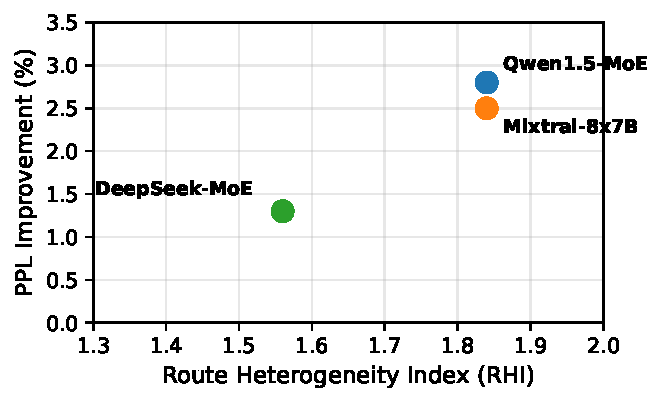
\includegraphics[width=0.48\textwidth]{figures/fig_rhi.pdf}
\caption{$\rhi$ vs.\ $\Delta$PPL at 2.5\,bits/param. Models with higher routing heterogeneity tend to benefit more from \method.}
\label{fig:rhi}
\end{figure}

\subsection{PPL Improvement Across Budgets}

Figure~\ref{fig:ppl_improve} visualizes the percentage PPL improvement as a function of bit budget. The aggressive regime (2.3--2.75\,bits) is shaded. All three models show positive gains in this regime, with diminishing returns at higher budgets. Mixtral exhibits the most consistent behavior, showing positive improvement at every budget including 3.0 and 3.25\,bits.

\begin{figure}[t]
\centering
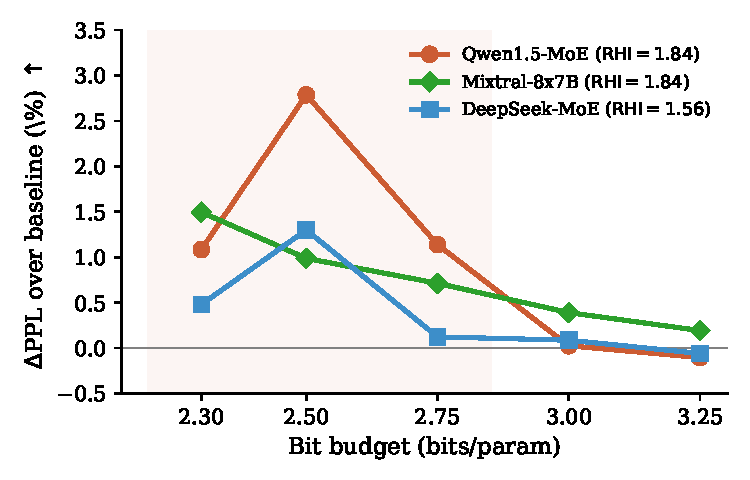
\includegraphics[width=0.48\textwidth]{figures/fig_ppl_improvement.pdf}
\caption{PPL improvement (\%) vs.\ bit budget across three models. \method\ improves over MxMoE in the aggressive regime (shaded), with all models showing positive gains.}
\label{fig:ppl_improve}
\end{figure}

\subsection{Allocation Analysis}

Figure~\ref{fig:alloc} compares the 2.5-bit allocation maps produced by the baseline and \method\ on Qwen1.5-MoE. Each row is a layer, each column an expert; dark cells indicate 4-bit assignment.

Quantitatively, RWS changes only 32 of 1{,}464 blocks (2.2\%) on Qwen at 2.5\,bits, yet reduces PPL by 2.8\%. The 24 blocks upgraded from W2 to W4 have mean routing frequency 364, while the 8 blocks downgraded from W4 to W2 have mean frequency 258 (overall mean: 273). On DeepSeek-MoE, 30 of 35 changed blocks are upgrades, with upgraded blocks averaging frequency 677 vs.\ 394 for downgraded blocks. RWS shifts precision toward higher-traffic experts, increasing the traffic-weighted average bits per activation from 2.079 to 2.112 (+0.034) on Qwen. The small number of changed blocks explains why the \emph{average} bits are nearly identical---RWS reallocates within the same budget, not by adding capacity.

\paragraph{Why small routing differences matter.}
Qwen1.5-MoE has near-uniform routing (entropy ratio 0.995), yet shows the largest PPL gain. The explanation lies in the ILP threshold effect: at 2.5\,bits, only ${\sim}$8\% of blocks receive W4. The ILP allocator ranks blocks by sensitivity and selects the top fraction. When many blocks have similar sensitivity scores---as is typical in well-trained models---small reweighting by routing frequency shifts blocks across the W4/W2 threshold. Among the 32 changed blocks, those upgraded by RWS have frequency $1.4\sigma$ above the layer mean, while downgraded blocks are at $-0.2\sigma$. Even a weak routing signal suffices to break ties among near-equal sensitivities.

\begin{figure}[t]
\centering
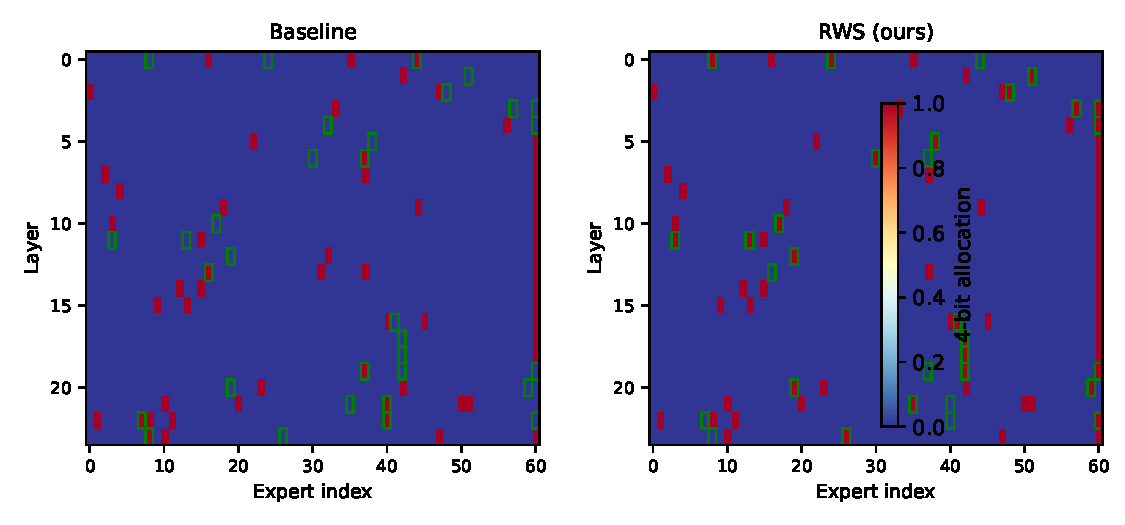
\includegraphics[width=0.48\textwidth]{figures/fig_allocation.pdf}
\caption{Allocation heatmaps at 2.5\,bits (Qwen1.5-MoE). Dark = W4A16, light = W2A16. Green borders mark blocks that differ between baseline and RWS.}
\label{fig:alloc}
\end{figure}

\subsection{Why Not Route-Only Allocation?}
\label{sec:freq-only}

A natural alternative to RWS is a \emph{frequency-only} allocation: assign 4-bit to the highest-traffic experts until the budget is met, ignoring sensitivity entirely. Figure~\ref{fig:freq_only} and Table~\ref{tab:freq_only} compare this baseline against MxMoE (sensitivity-only) and RWS across all three models. The results are unambiguous: frequency-only allocation fails catastrophically at aggressive budgets.

\begin{figure}[t]
\centering
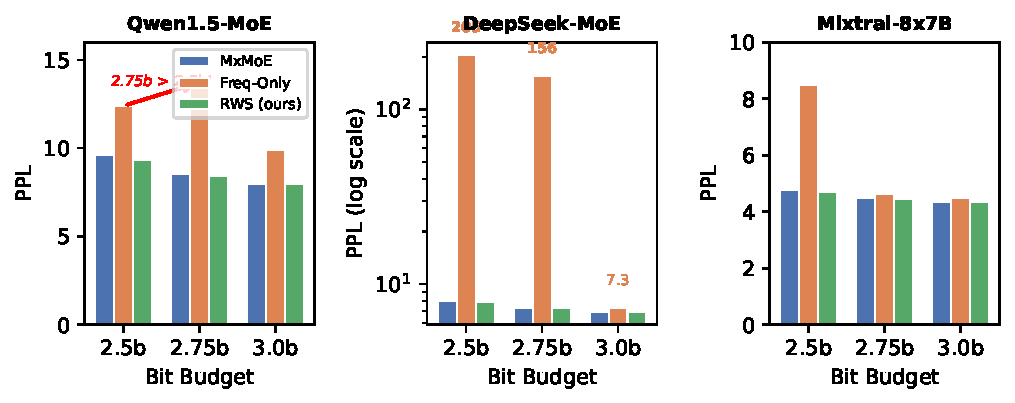
\includegraphics[width=0.48\textwidth]{figures/fig_freq_only.pdf}
\caption{Frequency-only vs.\ sensitivity-based allocation across three models. Freq-Only (orange) fails catastrophically at 2.5--2.75\,bits on DeepSeek (log scale) and shows non-monotonic behavior on Qwen (2.75b PPL $>$ 2.5b). RWS (green) consistently matches or improves upon MxMoE (blue).}
\label{fig:freq_only}
\end{figure}

\begin{table}[t]
\centering
\small
\caption{Frequency-only vs.\ sensitivity-based allocation. Freq-Only assigns W4 to the highest-traffic experts, ignoring sensitivity. \textbf{Bold}: best among three methods.}
\label{tab:freq_only}
\setlength{\tabcolsep}{3pt}
\begin{tabular}{llccc}
\toprule
Model & Method & Bits & Avg.$\uparrow$ & PPL$\downarrow$ \\
\midrule
\multirow{9}{*}{\textbf{Qwen}}
& MxMoE      & 3.00 & 63.8 &   7.95 \\
& Freq-Only  & 3.00 & 52.2 &   9.92 \\
& RWS (ours) & 3.00 & \textbf{63.9} & \textbf{7.95} \\
\cmidrule(lr){2-5}
& MxMoE      & 2.75 & 62.3 &   8.52 \\
& Freq-Only  & 2.75 & 43.7 &  13.72 \\
& RWS (ours) & 2.75 & \textbf{62.6} & \textbf{8.43} \\
\cmidrule(lr){2-5}
& MxMoE      & 2.50 & 59.5 &   9.62 \\
& Freq-Only  & 2.50 & 53.4 &  12.40 \\
& RWS (ours) & 2.50 & \textbf{60.2} & \textbf{9.35} \\
\midrule
\multirow{9}{*}{\textbf{DeepSeek}}
& MxMoE      & 3.00 & 64.4 &   6.93 \\
& Freq-Only  & 3.00 & 63.7 &   7.34 \\
& RWS (ours) & 3.00 & \textbf{64.6} & \textbf{6.93} \\
\cmidrule(lr){2-5}
& MxMoE      & 2.75 & 62.9 &   7.32 \\
& Freq-Only  & 2.75 & 26.9 & 155.54 \\
& RWS (ours) & 2.75 & \textbf{64.0} & \textbf{7.31} \\
\cmidrule(lr){2-5}
& MxMoE      & 2.50 & 61.0 &   8.01 \\
& Freq-Only  & 2.50 & 26.8 & 204.55 \\
& RWS (ours) & 2.50 & \textbf{61.1} & \textbf{7.90} \\
\midrule
\multirow{9}{*}{\textbf{Mixtral}}
& MxMoE      & 3.00 & 74.8 &   4.36 \\
& Freq-Only  & 3.00 & 74.2 &   4.48 \\
& RWS (ours) & 3.00 & \textbf{75.0} & \textbf{4.34} \\
\cmidrule(lr){2-5}
& MxMoE      & 2.75 & 72.8 &   4.49 \\
& Freq-Only  & 2.75 & 72.0 &   4.62 \\
& RWS (ours) & 2.75 & \textbf{73.1} & \textbf{4.46} \\
\cmidrule(lr){2-5}
& MxMoE      & 2.50 & 70.9 &   4.76 \\
& Freq-Only  & 2.50 & 63.4 &   6.19 \\
& RWS (ours) & 2.50 & \textbf{71.3} & \textbf{4.71} \\
\bottomrule
\end{tabular}
\end{table}

\paragraph{Frequency-only is consistently worse.}
Frequency-only allocation is worse than sensitivity-based allocation across all models and budgets (Table~\ref{tab:main}). The effect ranges from moderate (Mixtral 2.5b: PPL 6.19 vs.\ MxMoE 4.76, +30\%) to severe (DeepSeek 2.5b: PPL 204.6 vs.\ 8.01). On Qwen at 2.75\,bits, PPL degrades from 8.52 to 13.72 (+61\%), and paradoxically exceeds the 2.5\,bits result (12.40). Even at 3.0\,bits, frequency-only remains worse on all three models. Downstream accuracy follows the same pattern: DeepSeek 2.5\,bits drops to 26.8\% (vs.\ 61.0\% for MxMoE).

\paragraph{Frequency $\neq$ sensitivity.}
Why does frequency-only fail so dramatically? The allocation selects experts by \emph{how often} they are activated, not by \emph{how much they suffer} from low-bit quantization. In DeepSeek-MoE, each token is routed to 6 of 64 experts (top-6 gating). At 2.5\,bits, only 7 of 64 routed experts receive W4; the remaining 57 get W2. On average, each token encounters ${\sim}5.3$ W2 experts out of 6 selected---nearly every expert processing the token is poorly quantized. The frequency-based criterion allocates W4 to the most active experts, which tend to be \emph{robust} to quantization. The experts that are \emph{sensitive} to W2 quantization---those with high reconstruction error---are precisely the lower-frequency ones that frequency-only deprioritizes.

\paragraph{Non-monotonic behavior reveals the misalignment.}
On Qwen at 2.75\,bits, frequency-only yields \emph{worse} PPL (13.72) than at 2.5\,bits (12.40), despite allocating more W4 experts (14 vs.\ 5). This non-monotonicity is impossible under a correct allocation: adding more W4 should monotonically improve quality. It arises because expanding the W4 set from top-5 to top-14 by frequency adds experts that are high-frequency but \emph{low-sensitivity}, while some high-sensitivity experts remain at W2. Adding W4 to the wrong experts does not compensate for leaving sensitive experts at W2.

\paragraph{RWS combines both signals.}
\method\ resolves this by weighting sensitivity by routing frequency: $\hat{L} = L \cdot (1 + \pi/\max(\pi))$. Sensitivity identifies \emph{which} blocks suffer from W2 quantization; routing frequency prioritizes \emph{which} of those blocks matter most at inference. Neither signal alone suffices: sensitivity-only (MxMoE) ignores usage frequency and leaves marginal gains on the table, while frequency-only ignores quantization difficulty entirely and can be catastrophically wrong. The combination is strictly better than either component.

\paragraph{Scope.}
Our evidence supports \method\ for the specific setting of binary $\{$W2A16/G128, W4A16$\}$ strategy pools with RTN-based per-block quantization and sensitivity-based ILP allocation. We do not claim generalization to arbitrary mixed-precision pipelines, larger strategy pools, or alternative per-block quantization methods (GPTQ, AWQ) without testing. The binary strategy pool is chosen because RWS has the most leverage when the allocation is a binary choice---precisely the regime where \emph{which} experts receive the high-bit strategy matters. With a larger pool ($N > 2$ strategies), the allocator has more degrees of freedom and the marginal value of routing information may decrease; we leave this investigation to future work.

\subsection{Robustness and Limitations}

\paragraph{Calibration-subset sensitivity.}
To assess robustness to calibration data selection, we repeat the full calibration--allocation--evaluation pipeline with 3 different seeds for selecting 128 WikiText-2 samples. Table~\ref{tab:seed} reports the results. On both models, \method\ outperforms the baseline at every seed. The calibration-subset variance is small ($\sigma < 0.03$ PPL for both baseline and RWS) and the improvement direction is consistent: RWS improves PPL by 2.79--3.19\% on Qwen and 1.29--1.30\% on DeepSeek across all seeds.

\begin{table}[t]
\centering
\small
\caption{Calibration-subset sensitivity at 2.5\,bits. Three seeds for calibration data selection. RWS outperforms baseline at every seed on both models.}
\label{tab:seed}
\begin{tabular}{lcccc}
\toprule
& \multicolumn{2}{c}{Qwen} & \multicolumn{2}{c}{DeepSeek} \\
\cmidrule(lr){2-3} \cmidrule(lr){4-5}
Seed & Base. & RWS & Base. & RWS \\
\midrule
0 & 9.62 & \textbf{9.35} & 8.01 & \textbf{7.90} \\
1 & 9.65 & \textbf{9.37} & 8.04 & \textbf{7.93} \\
2 & 9.67 & \textbf{9.36} & 8.06 & \textbf{7.95} \\
\midrule
Mean & 9.65 & \textbf{9.36} & 8.03 & \textbf{7.93} \\
$\sigma$ & 0.025 & 0.010 & 0.025 & 0.025 \\
$\Delta$ & \multicolumn{2}{c}{$-$2.95\%} & \multicolumn{2}{c}{$-$1.30\%} \\
\bottomrule
\end{tabular}
\end{table}

\paragraph{Per-task analysis.}
Appendix~\ref{app:per-task} reports per-task accuracy for all three models at 2.5\,bits. RWS improves the 7-task average on all three models, but not every individual task: for example, ARC-Challenge on Qwen regresses from 37.7\% to 36.9\%. The improvements concentrate on LAMBADA (both variants) and HellaSwag, which are the most sensitive to token-level prediction quality---consistent with the hypothesis that routing-aware allocation improves the per-token output distribution.

\subsection{Hessian-Based Sensitivity: A Reference-Free Baseline}
\label{sec:hessian}

All methods compared so far require per-expert calibration data to measure quantization sensitivity. A natural question is whether a \emph{reference-free} metric---one that depends only on the model weights, not on input activations---can replace the reconstruction loss. We test this using Hessian trace sensitivity: for each expert, we approximate the trace of the diagonal Hessian via Hutchinson's method (50 random projections), sum across gate/up/down projections, and normalize per layer. We evaluate two variants:
\begin{itemize}
    \item \textbf{Hess-Only}: ranks experts by normalized Hessian trace, assigns W4 to the top-$k$.
    \item \textbf{Hess-RWS}: applies RWS weighting ($\hat{H} = H \cdot (1 + \pi/\max(\pi))$) before ranking.
\end{itemize}
Both use the same per-layer uniform budget and RTN quantization as MxMoE. Results are in Table~\ref{tab:main}.

\paragraph{Hessian underperforms reconstruction loss.}
Hessian-based allocation consistently trails reconstruction-loss-based allocation. On Qwen at 2.5\,bits, Hess-Only yields PPL\,=\,10.97 vs.\ MxMoE's 9.62 (+14\%); on DeepSeek, the gap is smaller but still significant (8.64 vs.\ 8.01, +8\%). Downstream accuracy follows: Hess-Only achieves only 53.7\% on Qwen (vs.\ MxMoE 59.5\%) and 60.0\% on DeepSeek (vs.\ 61.0\%).

\paragraph{Hessian sensitivity is nearly uniform across experts.}
The coefficient of variation (CV) of the normalized Hessian trace across experts within a layer averages only 2.1\% on Qwen and 4.4\% on DeepSeek. This near-uniformity means Hessian-based allocation struggles to differentiate experts, especially at low budgets where only a small fraction receive W4. The reconstruction loss captures activation-dependent effects that the weight-only Hessian cannot, providing a much stronger signal for allocation.

\paragraph{RWS helps Hessian more than it helps reconstruction loss.}
On Qwen at 3.0\,bits, RWS improves Hess-Only PPL by 3.4\% (9.43 $\to$ 9.11) but improves MxMoE by only 0.1\% (7.95 $\to$ 7.95). When the base sensitivity metric is noisy, routing information provides a stronger corrective signal. However, even Hess-RWS remains far below MxMoE (9.11 vs.\ 7.95), confirming that the choice of sensitivity metric matters more than the allocation weighting.

\subsection{Cross-Layer Propagation: A Cautionary Ablation}

A natural question is whether routing information can be \emph{propagated} across layers. We tested RouteQEP, which back-propagates per-expert reconstruction errors through the co-routing graph (Appendix~\ref{app:routeqep}). At 2.75\,bits on Qwen1.5-MoE: 1-hop propagation regresses PPL by 36\%, 2-hop by 51\%. The recursion amplifies the objective for highly connected expert pairs, causing the allocator to concentrate all high-bit slots on the most-connected experts regardless of their actual quantization sensitivity. This negative result supports our design choice of \emph{local} route weighting: routing information is valuable within a layer but harmful when naively propagated across layers. A principled normalization or attention-based aggregation may yet succeed, but the straightforward approach fails.

\section{Related Work}
\label{sec:related}

\paragraph{MoE architectures.}
Sparse MoE layers \citep{shazeer2017outrageously} enable massive parameter scaling with sub-linear compute growth. GShard \citep{lepikhin2021gshard} and Switch Transformers \citep{fedus2022switch} demonstrated scaling to billions of parameters. Recent models---Mixtral-8x7B \citep{jiang2024mixtral}, Qwen1.5-MoE \citep{bai2023qwen}, DeepSeek-V2/V3 \citep{deepseekai2024deepseekv2,deepseekai2024deepseekv3}, ST-MoE \citep{zoph2022stmoe}---use top-$k$ routing with shared and routed experts. Expert Choice routing \citep{zhou2022expertchoice} flips the assignment to let experts select tokens. Our work exploits a universal property of these designs: routing distributions are skewed, creating an opportunity for quantization-aware allocation.

\paragraph{LLM quantization.}
Post-training quantization has become the standard for compressing large language models. GPTQ \citep{frantar2023gptq} uses second-order Hessian information for layer-wise weight quantization. AWQ \citep{lin2024awq} identifies salient weight channels via activation magnitude. SmoothQuant \citep{xiao2023smoothquant} migrates quantization difficulty from activations to weights. LLM.int8() \citep{dettmers2022llmint8} and SpQR \citep{dettmers2024spqr} handle outlier features through mixed-precision decomposition. QLoRA \citep{dettmers2023qlora} couples quantization with parameter-efficient fine-tuning. Advanced codebook methods include QuIP/QuIP\# \citep{chee2024quip,tseng2024quipsharp}, AQLM \citep{egiazarian2024aqlm}, and OmniQuant \citep{shao2024omniquant}. These methods are orthogonal to the allocation problem we study; \method\ is composable with any per-block quantization algorithm.

\paragraph{Mixed-precision allocation.}
The HAWQ family \citep{dong2019hawq,yao2021hawqv3} uses sensitivity-based mixed-precision for CNNs and Transformers, with HAWQ-V3 introducing ILP-based allocation. MxMoE \citep{duanmu2025mxmoe} extends this to MoE with hardware-aware GroupGEMM kernels. QuantMoE-Bench \citep{li2024quantmoebench} benchmarks MoE quantization methods. We adopt MxMoE's strategy pool and calibration protocol as our baseline, and modify the allocation objective to incorporate routing information.

\paragraph{MoE-specific compression.}
QMoE \citep{frantar2023qmoe} applies sub-bit dictionary coding to MoE weights. EAC-MoE \citep{chen2025eacmoe} compresses expert activations. MoE-Pruning \citep{yang2024moei2} and Sparse Upcycling \citep{komatsuzaki2023sparseupcycling} reduce expert count. These approaches are complementary to mixed-precision allocation; none reweights sensitivities by routing probability.

\paragraph{Routing analysis.}
Prior work studies MoE routing for load balancing \citep{fedus2022switch}, capacity factor tuning, and expert specialization \citep{zhou2022expertchoice}. To our knowledge, we are the first to exploit routing skew in the \emph{objective} of a post-training quantization allocator and to propose a heterogeneity-based diagnostic for when such exploitation is beneficial.
\section{Conclusion}

We have identified a specific, correctable mismatch in MoE mixed-precision quantization: sensitivity-based allocators treat every expert's reconstruction loss equally, ignoring that routing frequencies vary by orders of magnitude. Route-Weighted Sensitivity corrects this by scaling each expert's sensitivity by its routing weight before the ILP---a modification to the objective that is principled (approximating the expected inference loss), conservative (bounded $2\times$ scaling), and effective (consistent PPL improvements on all three models at aggressive budgets). The method requires no tuning and no additional calibration cost. The Route Heterogeneity Index ($\rhi$) provides a cheap preliminary indicator of whether routing-aware allocation is worth trying.

Our cross-layer ablation shows that naive propagation of routing information fails catastrophically, supporting the design choice of local, per-layer route weighting. The broader lesson is that \emph{the allocator objective should reflect how often a weight is used at inference}; future MoE compression work could extend this principle to latency profiles, outlier smoothing, and activation-aware sensitivity.

\paragraph{Limitations.}
Our claims are deliberately scoped: \method\ is evaluated with a binary strategy pool and RTN-based per-block quantization; generalization to larger strategy pools and GPTQ/AWQ-based methods requires testing. The $(1 + w)$ weighting is a conservative heuristic; systematic comparison with raw-$\piprob$, gate-mass, and conditional-loss weighting across all models would further validate the design. RHI is presented as a preliminary diagnostic with only three data points; additional models are needed to confirm its utility. Calibration-subset sensitivity across 3 seeds confirms consistent improvements (Table~\ref{tab:seed}), though more seeds and diverse calibration sources would strengthen robustness claims.


\bibliographystyle{acl_natbib}
\bibliography{references}

\appendix
\section{Per-Task Downstream Breakdowns}
\label{app:per-task}

\begin{table*}[h]
\centering
\small
\setlength{\tabcolsep}{3pt}
\caption{Per-task accuracy at 2.5\,bits/param for all three models. \textbf{Bold}: RWS improvement.}
\begin{tabular}{l cc cc cc}
\toprule
& \multicolumn{2}{c}{Qwen1.5-MoE} & \multicolumn{2}{c}{Mixtral-8x7B} & \multicolumn{2}{c}{DeepSeek-MoE} \\
\cmidrule(lr){2-3} \cmidrule(lr){4-5} \cmidrule(lr){6-7}
Task & Base. & RWS & Base. & RWS & Base. & RWS \\
\midrule
PIQA            & 75.4 & \textbf{75.8} & 79.3 & \textbf{79.7} & 74.9 & \textbf{75.2} \\
HellaSwag       & 69.5 & \textbf{70.1} & 80.4 & \textbf{80.9} & 70.2 & 69.9 \\
ARC-Easy        & 58.1 & \textbf{59.3} & 75.8 & \textbf{76.2} & 63.7 & 63.4 \\
ARC-Challenge   & 37.7 & 36.9          & 52.0 & \textbf{52.3} & 39.1 & 38.9 \\
WinoGrande      & 63.4 & 63.0          & 71.9 & \textbf{72.3} & 63.2 & \textbf{63.9} \\
LAMBADA-OpenAI  & 59.3 & \textbf{61.3} & 71.7 & \textbf{72.1} & 61.1 & \textbf{61.3} \\
LAMBADA-Std     & 53.2 & \textbf{54.6} & 65.2 & \textbf{65.6} & 54.8 & \textbf{55.1} \\
\midrule
Average         & 59.5 & \textbf{60.2} & 70.9 & \textbf{71.3} & 61.0 & \textbf{61.1} \\
\bottomrule
\end{tabular}
\end{table*}

\section{Allocation Artifacts}
\label{app:allocation}

We release per-layer ILP allocations for all three models at all five budgets under both the baseline and \method. Allocation heatmaps for Qwen1.5-MoE at 2.5\,bits are shown in Figure~\ref{fig:alloc}.

\section{RouteQEP Negative-Result Details}
\label{app:routeqep}

RouteQEP extends \method\ by propagating quantization errors across layers through the co-routing graph. Let $\delta_{l,e}$ be the local quantization error for expert $e$ at layer $l$. RouteQEP defines a propagated error:
\begin{equation}
\tilde{\delta}_{l,e} = \delta_{l,e} + \lambda \sum_{e'} \Pr\!\bigl(e' \mid e,\, l{+}1\bigr)\, \tilde{\delta}_{l+1,e'},
\end{equation}
where $\Pr(e' \mid e, l)$ is the empirical co-routing probability---the fraction of tokens routed to $e$ at layer $l$ that are also routed to $e'$ at layer $l{+}1$.

The issue is that the co-routing probability $\Pr(e' \mid e)$ can be high for popular expert pairs, causing the recursion to amplify local errors rather than averaging them out. Specifically, the expected amplification per hop is roughly $\lambda \cdot \bar{c}$, where $\bar{c}$ is the mean co-routing probability over all expert pairs. With $\lambda\!=\!1$ and $\bar{c}$ typically in the range 0.1--0.3, the 1-hop propagated error is 1.1--1.3$\times$ the local error, and higher hops accumulate. The allocator responds to this amplified objective by concentrating all high-bit slots on the most-connected experts, regardless of their actual quantization sensitivity.

Results at 2.75\,bits on Qwen1.5-MoE:
\begin{itemize}
\item \textbf{No propagation} (\method, local): PPL 8.43 (baseline 8.52).
\item \textbf{1-hop} ($\lambda\!=\!1.0$): PPL 11.54 ($+$36\% vs.\ baseline).
\item \textbf{2-hop} ($\lambda\!=\!1.0$): PPL 12.87 ($+$51\% vs.\ baseline).
\item \textbf{1-hop normalized} (divide by depth): PPL 10.51 ($+$23\%).
\end{itemize}

All variants regress PPL. The allocator is responding rationally to an objective that over-weights highly connected experts. We conclude that intra-layer routing information is valuable but naive recursive cross-layer propagation is not with this formulation.


\end{document}
